\clearpage

\section{M-QAM Transmitter}

\begin{tcolorbox}	
	\begin{tabular}{p{2.75cm} p{0.2cm} p{10.5cm}} 	
		\textbf{Header File}   &:& m\_qam\_transmitter.h \\
		\textbf{Source File}   &:& m\_qam\_transmitter.cpp \\
        \textbf{Version}       &:& 20180815 (\emph{Filipa Simoes})\\
	\end{tabular}
\end{tcolorbox}

This block generates a MQAM optical signal. It can also output the binary sequence. A schematic representation of this block is shown in figure \ref{MQAM_transmitter_block_diagram_simple}.

\begin{figure}[h]
	\centering
	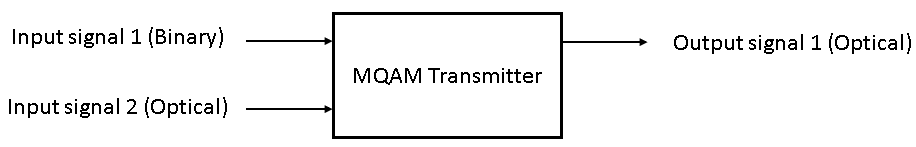
\includegraphics[width=0.6\textwidth]{./lib/m_qam_transmitter/figures/MQAM_transmitter_block_diagram_simple}
	\caption{Basic configuration of the MQAM transmitter}\label{MQAM_transmitter_block_diagram_simple}
\end{figure}

\subsection*{Functional description}

This block generates an optical signal (output signal 1 in figure \ref{MQAM_transmitter_block_diagram}). The binary signal generated in the internal block Binary Source (block B1 in figure \ref{MQAM_transmitter_block_diagram}) can be used to perform a Bit Error Rate (BER) measurement and in that sense it works as an extra output signal (output signal 2 in figure \ref{MQAM_transmitter_block_diagram}).

\begin{figure}[h]
	\centering
	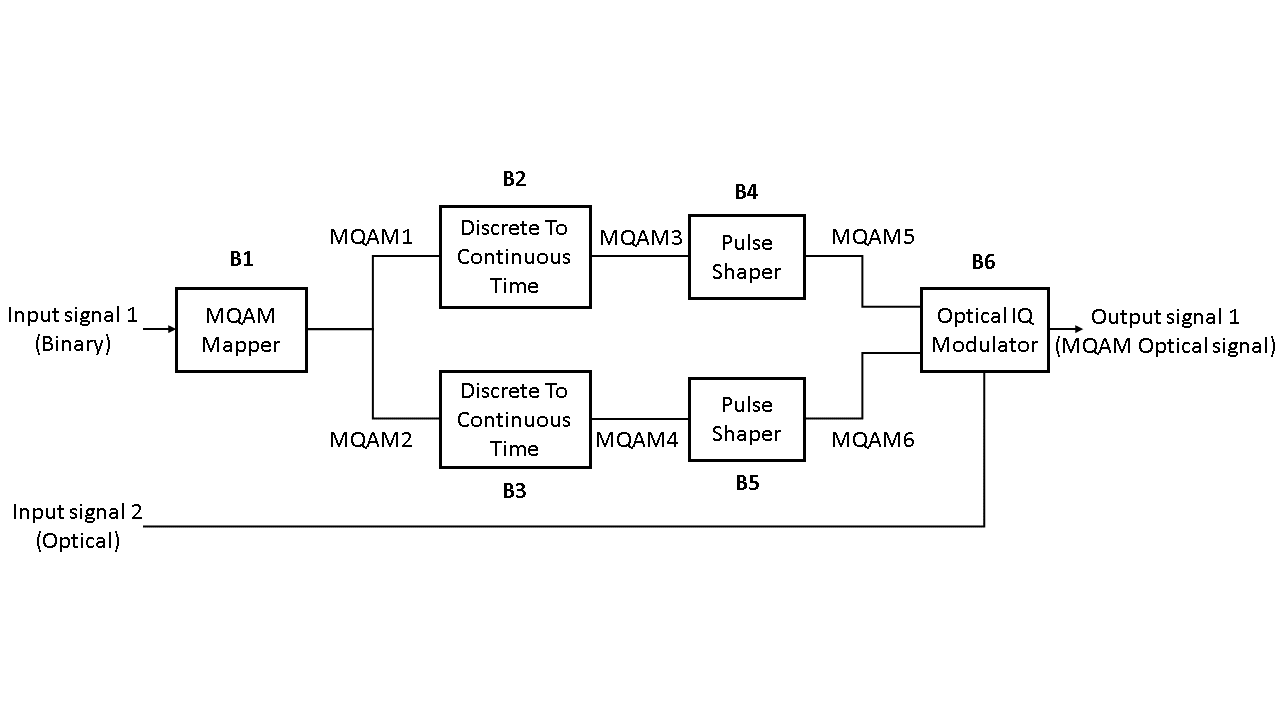
\includegraphics[width=\textwidth]{./lib/m_qam_transmitter/figures/MQAM_transmitter_block_diagram}
	\caption{Schematic representation of the block MQAM transmitter.}\label{MQAM_transmitter_block_diagram}
\end{figure}

\subsection*{Input parameters}

This block has a special set of functions that allow the user to change the basic configuration of the transmitter. The list of input parameters, functions used to change them and the values that each one can take are summarized in table \ref{table}.

\begin{table}[h]
\begin{center}
	\begin{tabular}{| m{3cm} | m{6cm} |  m{2cm} | m{4,3cm} | }
		\hline
		\textbf{Input parameters} & \textbf{Function} & Type & \textbf{Accepted values} \\ \hline
		Mode & setMode() & string & PseudoRandom \newline Random \newline DeterministicAppendZeros \newline DeterministicCyclic \\ \hline
		Number of bits generated & setNumberOfBits() & int & Any integer\\ \hline
		Pattern length & setPatternLength() & int & Real number greater than zero\\ \hline
		Number of bits & setNumberOfBits() & long & Integer number greater than zero\\ \hline
		Number of samples per symbol & setNumberOfSamplesPerSymbol() & int & Integer number of the type $2^n$ with n also integer\\ \hline
		Roll of factor & setRollOfFactor() & double & $\in$ [0,1] \\ \hline
		IQ amplitudes & setIqAmplitudes() & Vector of coordinate points in the I-Q plane & \textbf{Example} for a 4-qam mapping: \{ \{ 1.0, 1.0 \}, \{ -1.0, 1.0 \}, \{ -1.0, -1.0 \}, \{ 1.0, -1.0 \} \} \\ \hline
		Output optical power & setOutputOpticalPower() & int & Real number greater than zero\\ \hline
		Save internal signals & setSaveInternalSignals() & bool & True or False\\
		\hline
	\end{tabular}
	\caption{List of input parameters of the block MQAM transmitter} \label{table}
\end{center}
\end{table}

%\begin{itemize}
%	\item setMode(PseudoRandom);
%	\item setBitPeriod(1.0/50e9);
%	\linebreak (double)
%	\item setPatternLength(3);
%	\linebreak (int)
%	\item setNumberOfBits(10000);
%	\linebreak (long)
%	\item setNumberOfSamplesPerSymbol(32);
%	\linebreak (int)
%	\item setRollOffFactor(0.9);
%	\linebreak (double $\in$ [0,1])
%	\item setIqAmplitudes(\{ \{ 1, 1 \}, \{ -1, 1 \}, \{ -1, -1 \}, \{ 1, -1 \} \});
%	\item setOutputOpticalPower\_dBm(0);
%	\item setSaveInternalSignals(true);
%\end{itemize}

\pagebreak

\subsection*{Methods}

MQamTransmitter(vector$<$Signal *$>$ \&inputSignal, vector$<$Signal *$>$ \&outputSignal); (\textbf{constructor})
\bigbreak

void set(int opt);
\bigbreak
void setMode(BinarySourceMode m)
\bigbreak
BinarySourceMode const getMode(void)
\bigbreak
void setProbabilityOfZero(double pZero)
\bigbreak
double const getProbabilityOfZero(void)
\bigbreak
void setBitStream(string bStream)
\bigbreak
string const getBitStream(void)
\bigbreak
void setNumberOfBits(long int nOfBits)
\bigbreak
long int const getNumberOfBits(void)
\bigbreak
void setPatternLength(int pLength)
\bigbreak
int const getPatternLength(void)
\bigbreak
void setBitPeriod(double bPeriod)
\bigbreak
double const getBitPeriod(void)
\bigbreak
void setM(int mValue)
int const getM(void)
\bigbreak
void setIqAmplitudes(vector$<$t\textunderscore iqValues$>$ iqAmplitudesValues)
\bigbreak
vector$<$t\textunderscore iqValues$>$ const getIqAmplitudes(void)
\bigbreak
void setNumberOfSamplesPerSymbol(int n)
\bigbreak
int const getNumberOfSamplesPerSymbol(void)
\bigbreak
void setRollOffFactor(double rOffFactor)
\bigbreak
double const getRollOffFactor(void)
\bigbreak
void setSeeBeginningOfImpulseResponse(bool sBeginningOfImpulseResponse)
\bigbreak
double const getSeeBeginningOfImpulseResponse(void)
\bigbreak
void setOutputOpticalPower(t\textunderscore real outOpticalPower)
\bigbreak
t\textunderscore real const getOutputOpticalPower(void)
\bigbreak
void setOutputOpticalPower\_dBm(t\_real outOpticalPower\_dBm)
\bigbreak
t\_real const getOutputOpticalPower\_dBm(void)
\pagebreak

\subsection*{Output Signals}

\subparagraph*{Number:} 1 optical and 1 binary (optional)

\subparagraph*{Type:} Optical signal

\subsection*{Example}

\subsection*{Relevant Aspects}
1)Cardinality of the constellation: The constellation has 4 points, and the cardinality has an impact on the number of bits per symbol that can be sent: closer symbols in the constellation increase the probability of error.\\
2)Constellation coding :gray encoding, which allows the representation of two integers i and i + 1 to differ only in one bit.\\ 
3)Pulse shape: The impulse response is shown below (Analysis of the transmitter block)\\ 
4)Impact of a finite impulse response (pulse shaper):Pulse shaper applies an electrical filter to the signal. The fact that the number of samples per symbol is finite allows that we can specify the total duration of the pulse sequence, the frequency ranges is desired to perturb, the desired perturbation and the frequency range is desired not to perturb. Then is possible minimize the error probability.\\
5)Signal bandwidth: The signal bandwith is related to IES: As the bandwith decreases, the IES increases.\\
6)Inter symbolic interference: In the transmitter block IES=0.

\subsection*{Analysis of the transmitter block}
\subsection*{Binary Source}
Generates a sequence of binary values (1 or 0). The mode parameter allows the selection of the operation mode of the binary source (Random Mode; Pseudorandom Mode; DeterministicCyclic Mode and DeterministicAppendZeros Mode).\\
Example:
\begin{figure}[h]
	\centering
	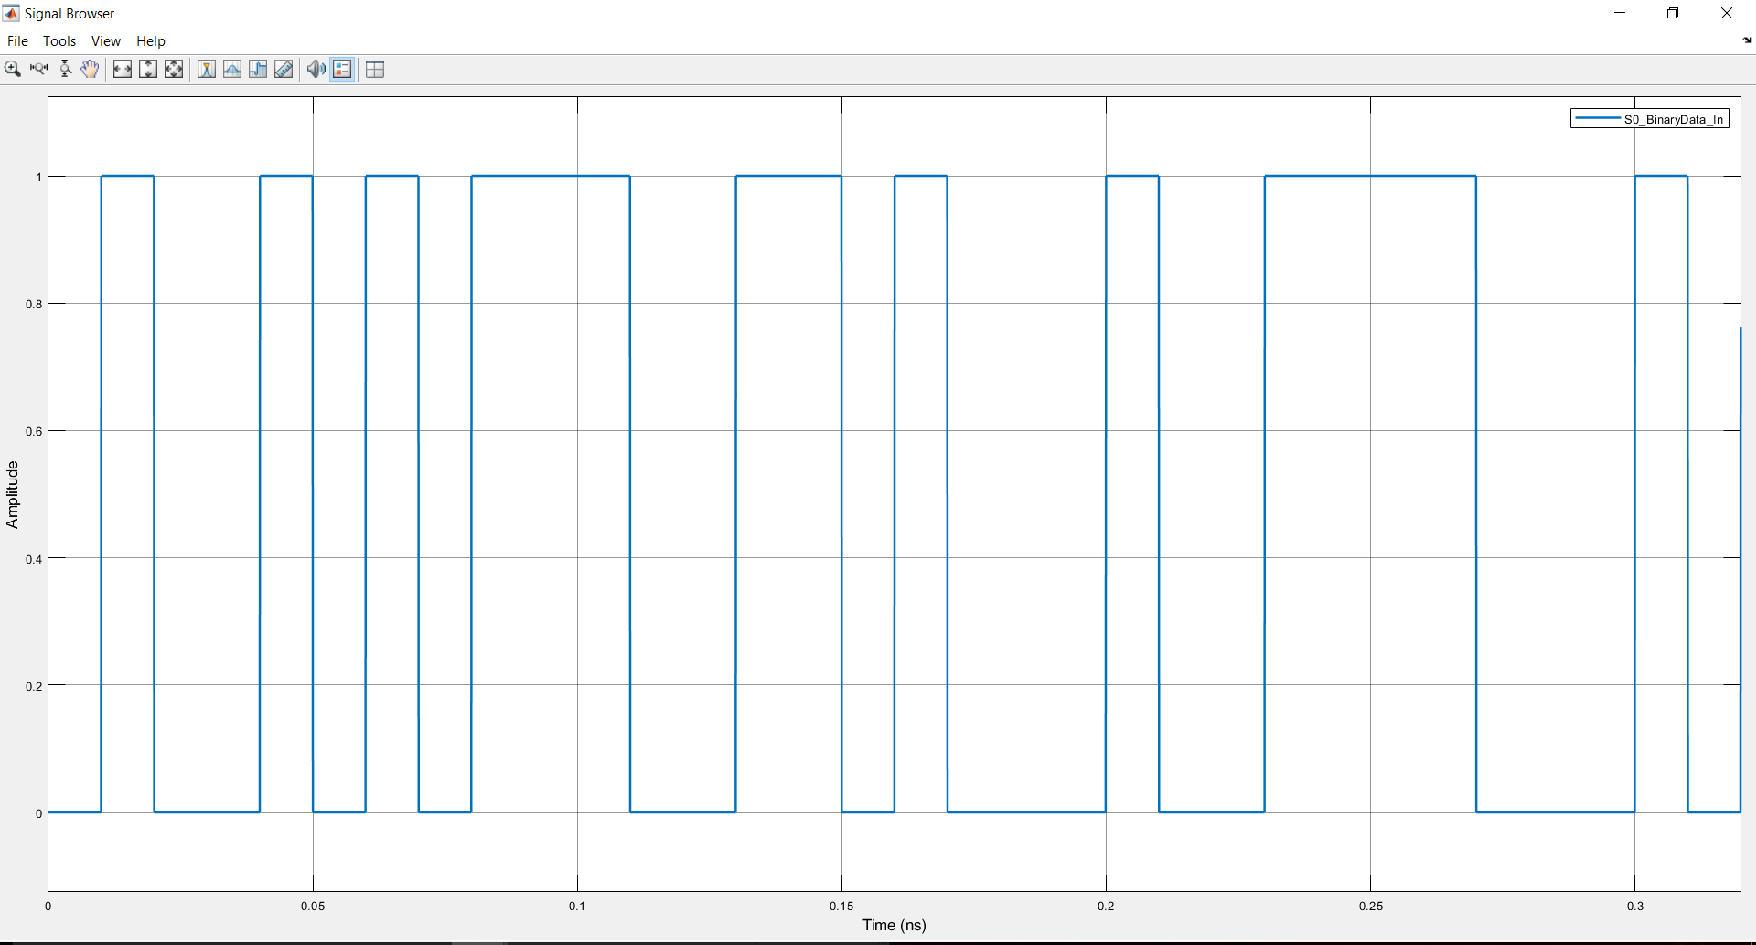
\includegraphics[width=1\textwidth]{../lib/m_qam_transmitter/figures/S0.pdf}
	\caption{Binary Source Output}\label{fig:Binary Source Output}
\end{figure}

Binary Source Output(S0): 01001010111001101000100111100010
\subsection*{M QAM MAPPER}
Example:
\begin{figure}[h]
	\centering
	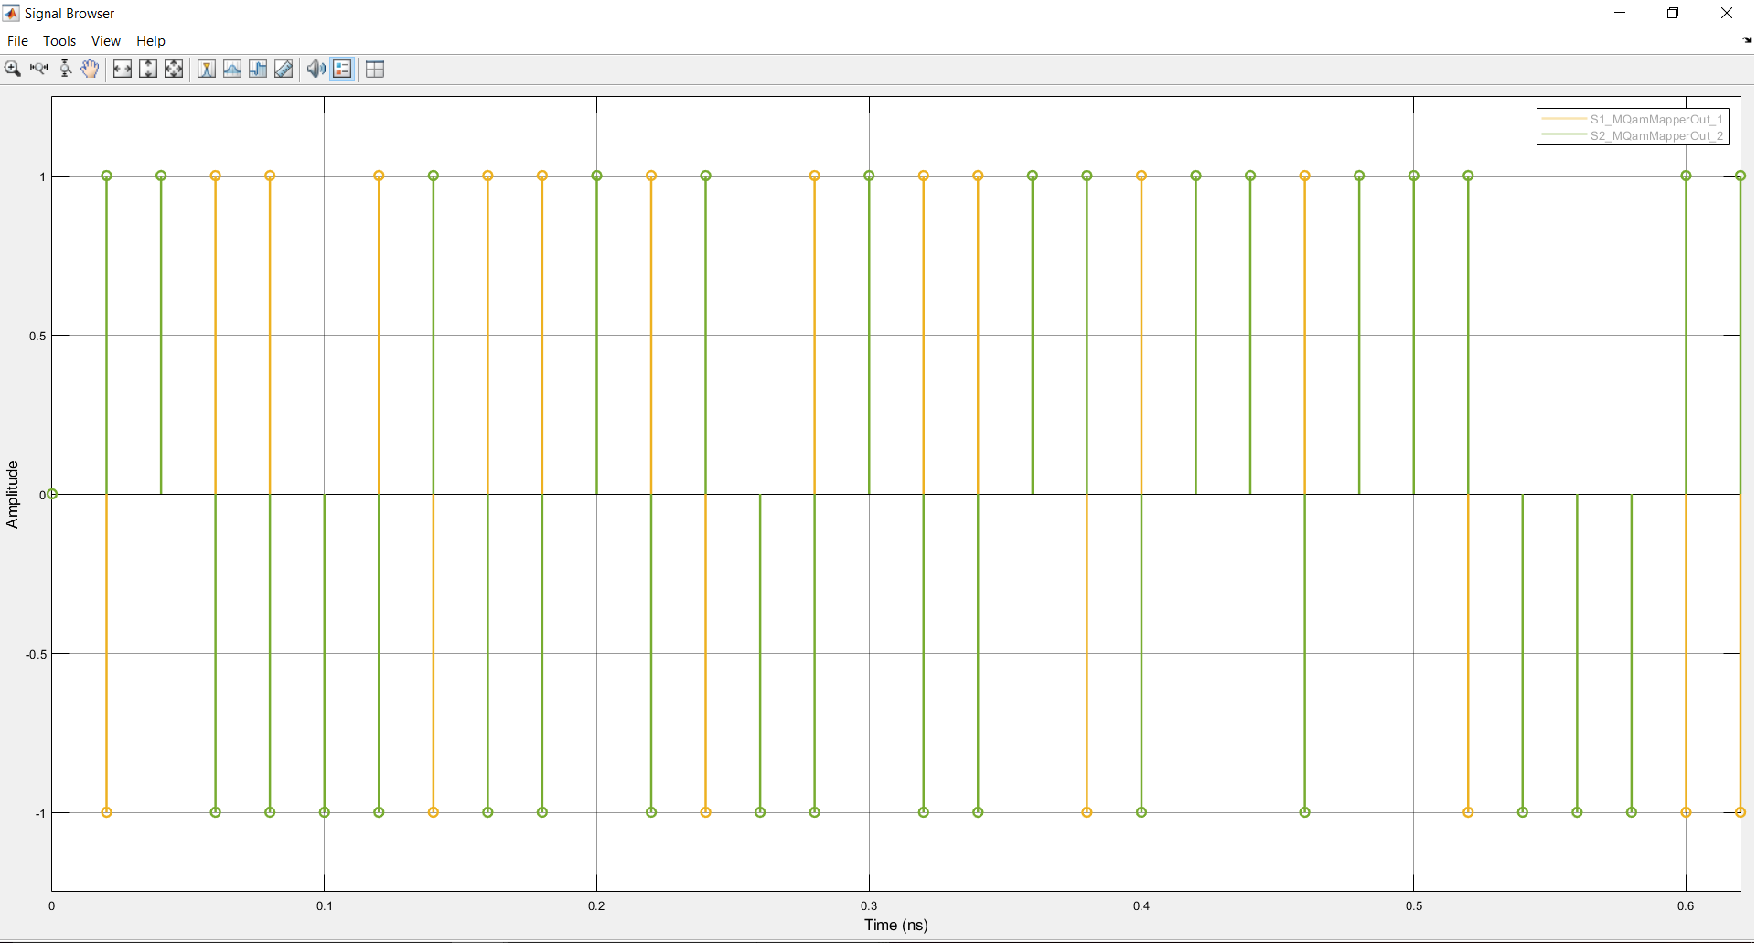
\includegraphics[width=1\textwidth]{../lib/m_qam_transmitter/figures/S1_S2.pdf}
	\caption{M QAM MAPPER Output}\label{fig:M QAM MAPPER Output}
\end{figure}

M-QAM MAPPER output: \\
S1(I): -1;1;1;1;-1;1;-1;1;1;1;1;-1;-1;1;1;1\\
S2(Q): 1;1;-1;-1;-1;-1;1;-1;-1;1;-1;1;-1;-1;1;-1\\

\subsection*{Discrete to Continuous Time}
Allows the conversion of a signal discrete in time to a continuous signal in time.
Example:

\begin{figure}[h]
	\centering
	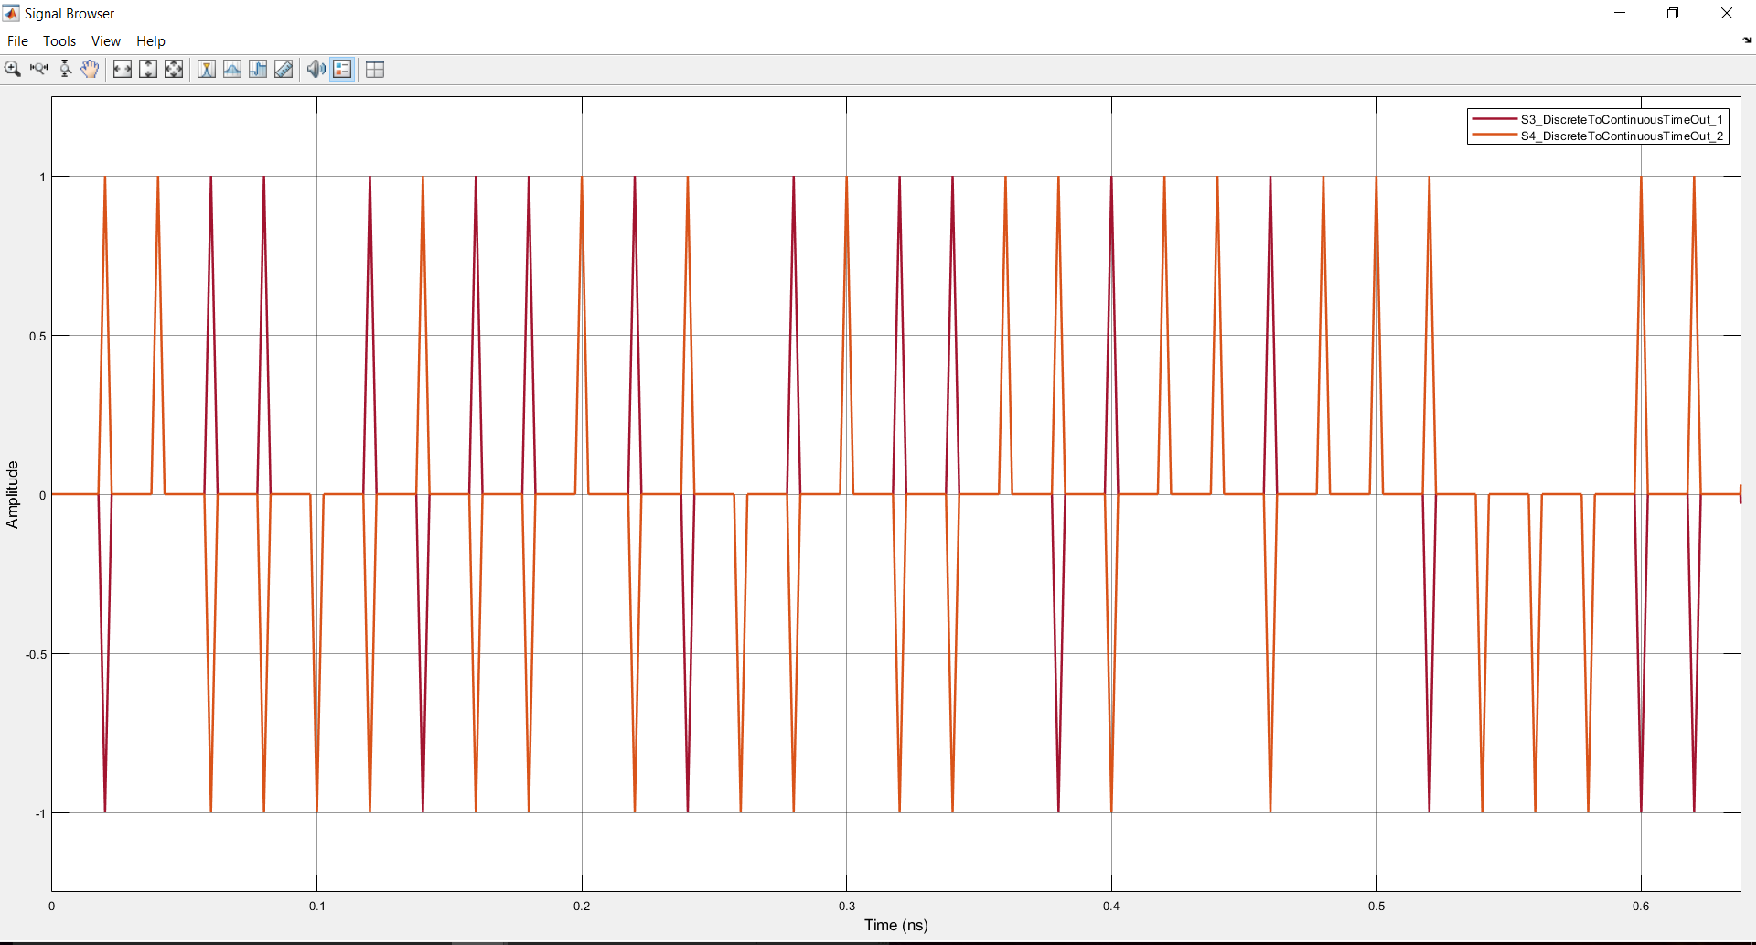
\includegraphics[width=1\textwidth]{../lib/m_qam_transmitter/figures/S3_S4.pdf}
	\caption{Discrete To Continuous Time}\label{fig:Discrete To Continuous Time}
\end{figure}

TimeToContinuous output: \\
S3(I): -1;1;1;1;-1;1;-1;1;1;1;1;-1;-1;1;1;1\\
S4(Q): 1;1;-1;-1;-1;-1;1;-1;-1;1;-1;1;-1;-1;1;-1\\
Eye Diagram: The open eye is large; IES=0;
Example:
\begin{figure}[h]
	\centering
	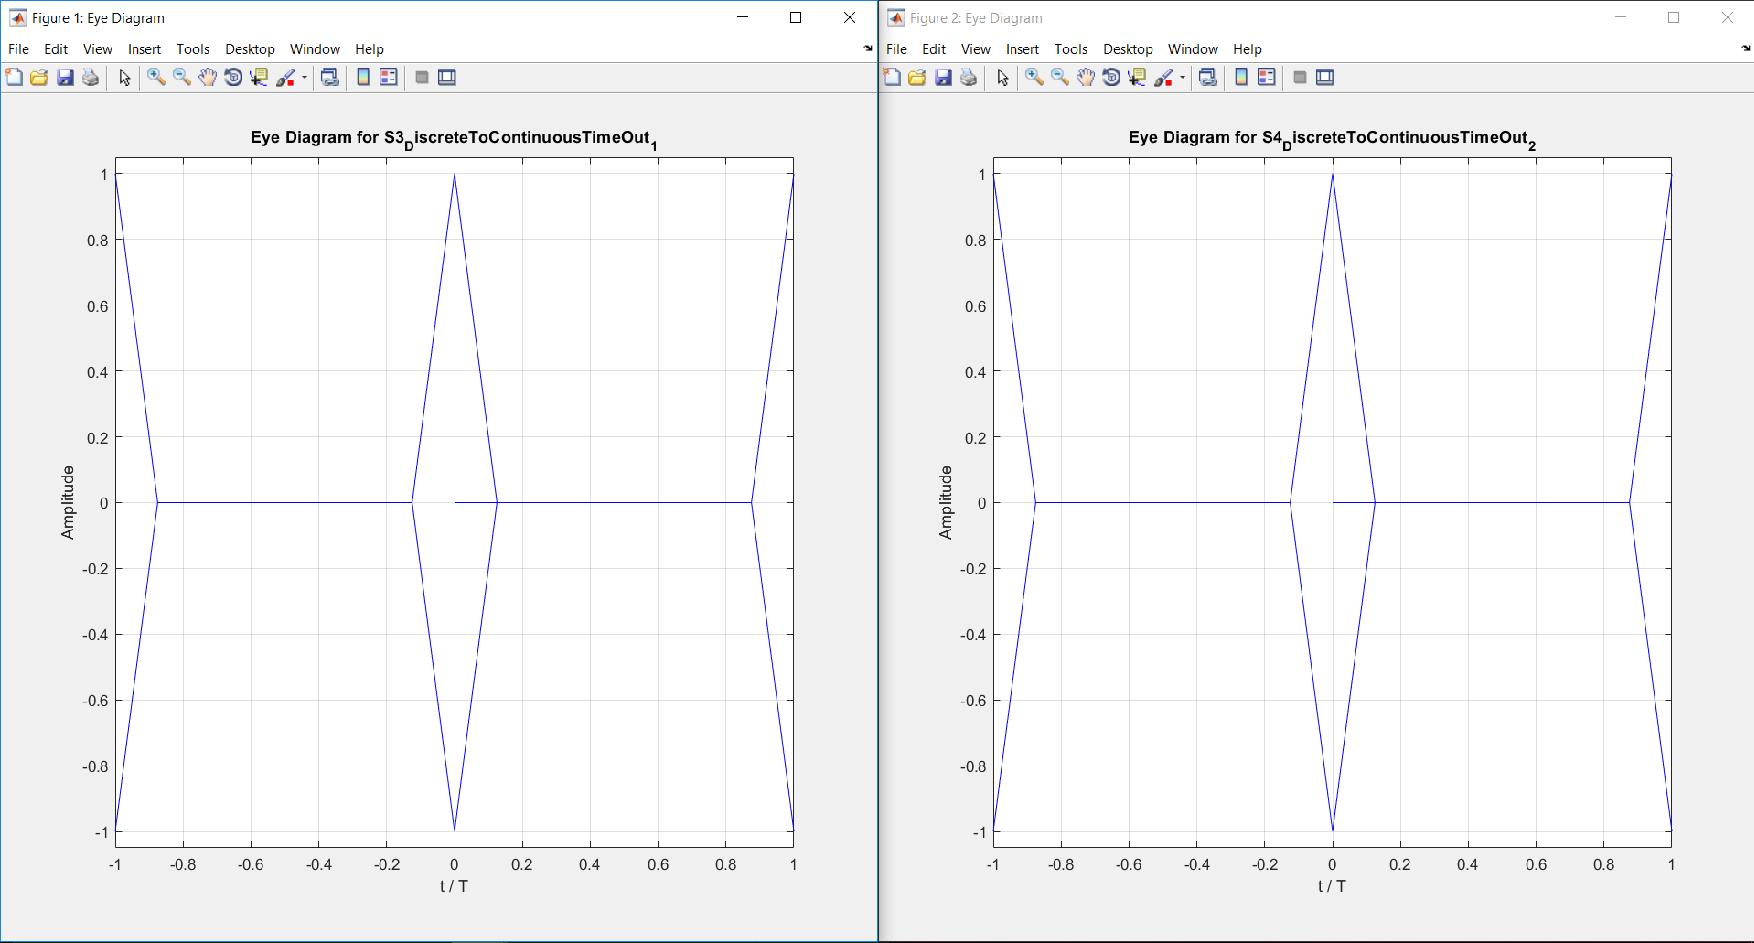
\includegraphics[width=1\textwidth]{../lib/m_qam_transmitter/figures/S3_S4_eye.pdf}
	\caption{Discrete To Continuous Time: Eye Diagram}\label{fig:Discrete To Continuous Time: Eye Diagram}
\end{figure}
\subsection*{Pulse Shaper}
Applies an electrical filter to the signal(input signal: sequence of Dirac delta functions; output signal continuous in time and in amplitude).
Example:
\begin{figure}[h]
	\centering
	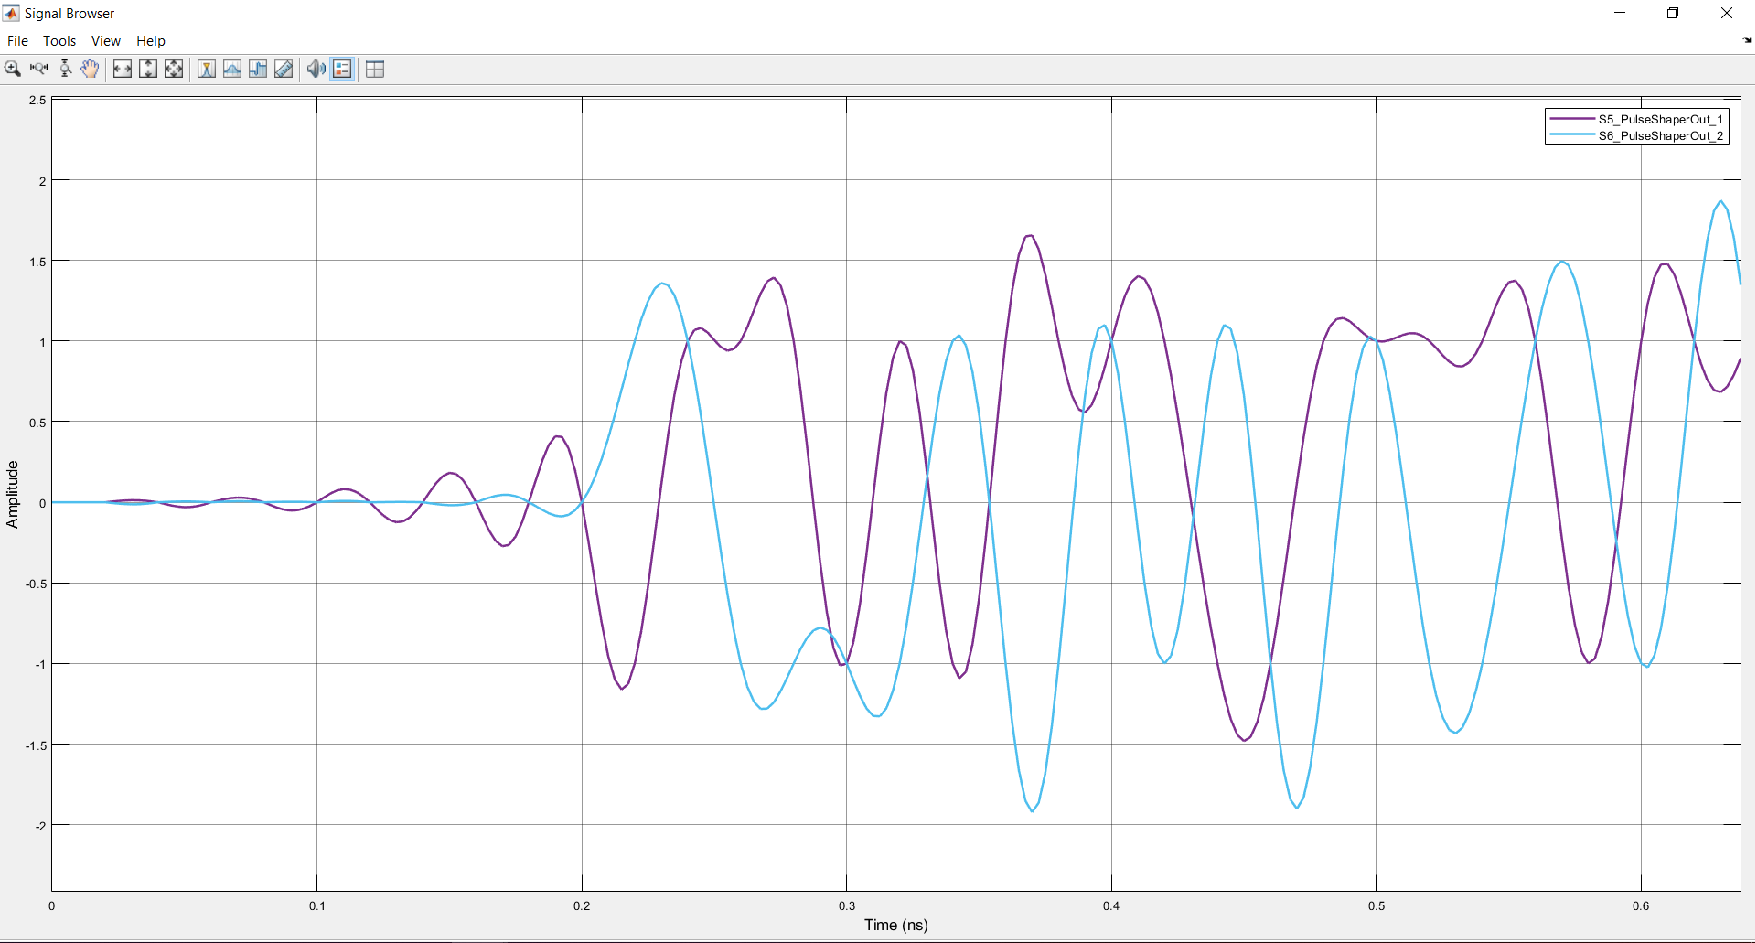
\includegraphics[width=1\textwidth]{../lib/m_qam_transmitter/figures/S5_S6.pdf}
	\caption{Impulse response I(t)and Q(t)}\label{fig:Impulse response I(t)and Q(t)}
\end{figure}

Eye diagram:the eye opening is large; IES=0.
\begin{figure}[h]
	\centering
	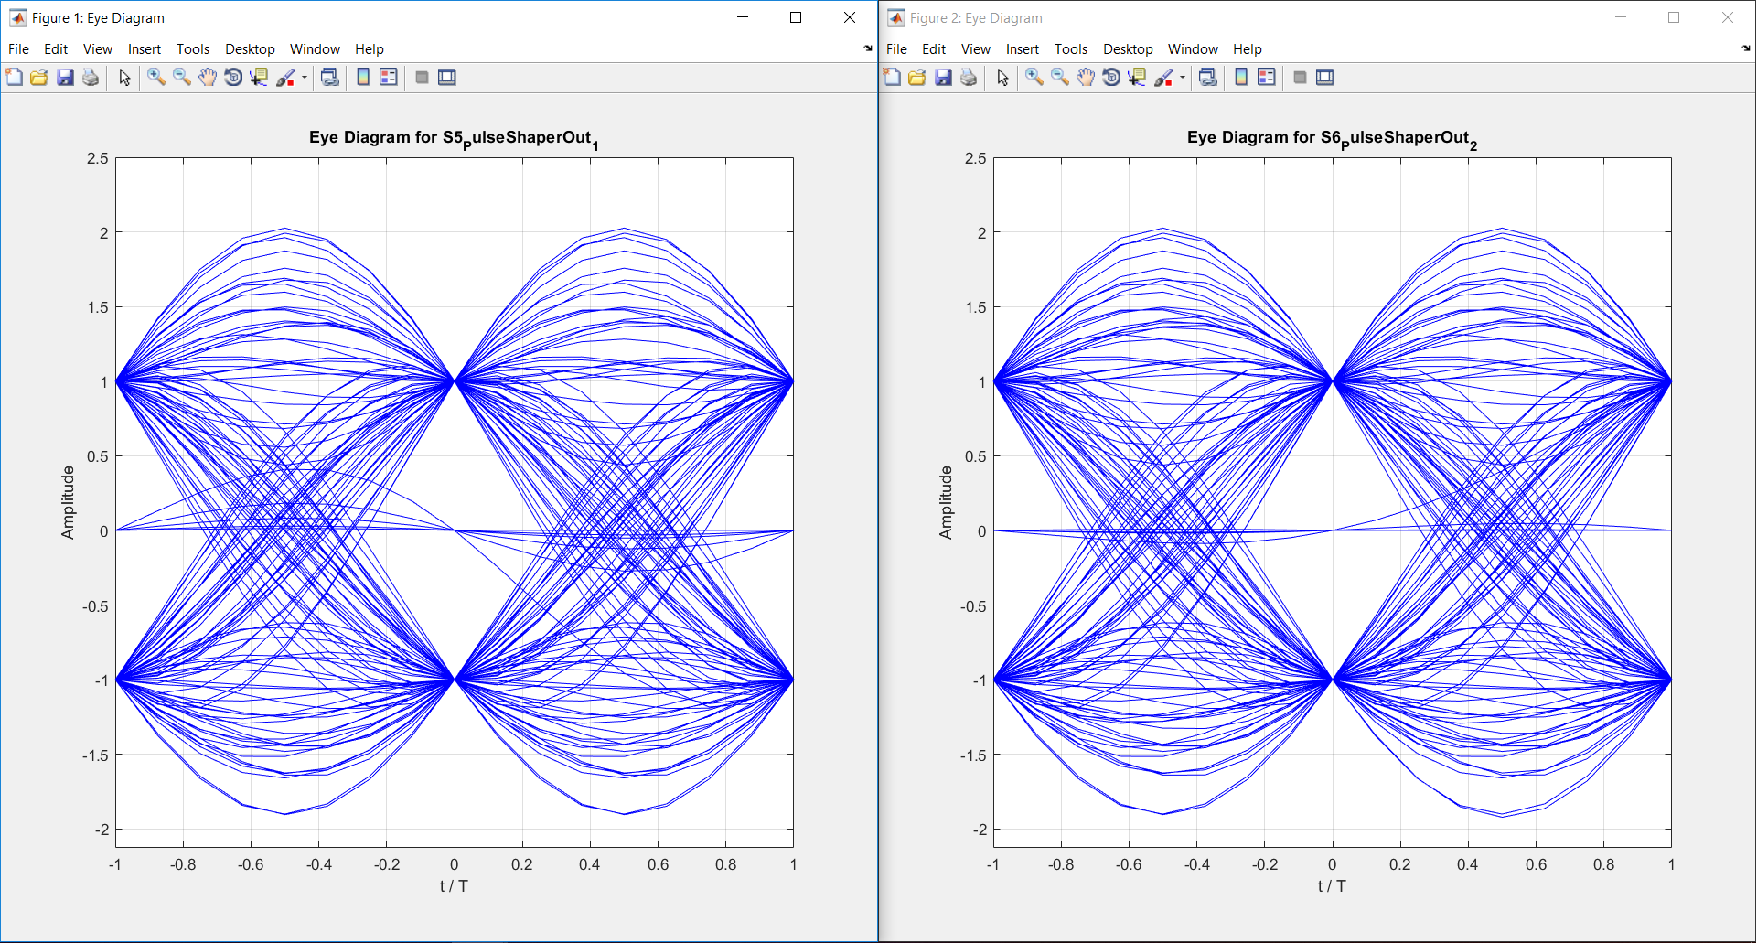
\includegraphics[width=1\textwidth]{../lib/m_qam_transmitter/figures/S5_S6_eye.pdf}
	\caption{Eye Diagram}\label{fig:eye}
\end{figure}

\subsection*{IQ Modulator}
Input signal continuous in time and amplitude; output signals: an optical signal and a binary signal.
Example:
\begin{figure}[h]
	\centering
	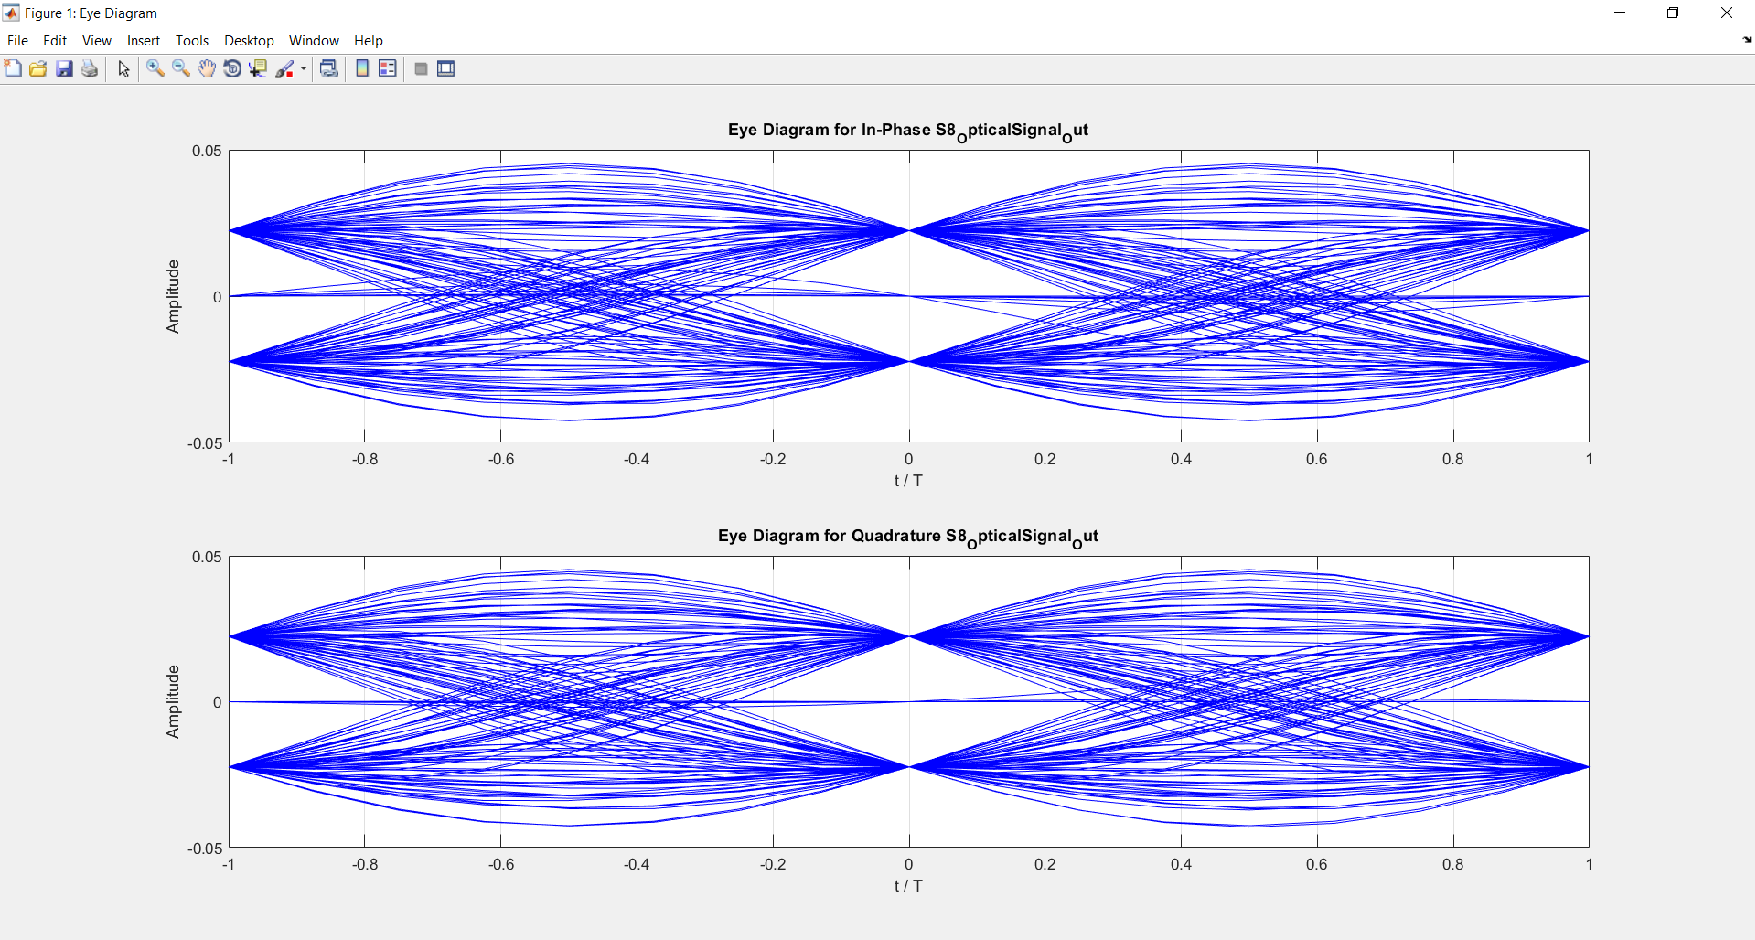
\includegraphics[width=1\textwidth]{../lib/m_qam_transmitter/figures/S8_eye.pdf}
	\caption{IQ Modulator output: eye diagram}\label{fig:IQ Modulator output: eye diagram}
\end{figure}

Eye diagram: As expected,the receiver block has an IES of zero.

\subsection*{Sink}
Accepts an input signal and it does not produce output signals. It takes
samples out of the buffer until the buffer is empty.



%\subsection*{Sugestions for future improvement}

%Add to the system another block similar to this one in order to generate two optical %signals with perpendicular polarizations. This would allow to combine the two optical %signals and generate an optical signal with any type of polarization.
